% Bedienungsanleitung für Clients

%\epigraph{	Your Time is precius. \newline Track your investments!}{\textit{Group 4}} %Raus mit dem kleinen Scherz??
\section{Bedienungsanleitung des Clients}
% So schön mit Bildern und so, erst bei fertiger Anwendung 

\begin{center}
	\textit{Your Time is precious. \newline Track your investments!}
\end{center}


TimeTracker bietet folgende Funktionen:
\begin{itemize}
	\item Time Tracking
	\item Anlegen und Löschen von Aktivitäten % durch User
	\item Tracking für verschiedene Aktivitäten
	\item Zuordnen mit Tags
	\item Abruf von Statistiken (Benutzer/Global)
\end{itemize}


Der Dienst ist online zu erreichen unter \url{https://iamtrent.de}
Lokale Installationen sind zu erreichen unter \url{localhost}

\subsection{Build}

Um die Anwendung zu bauen und lokal hochzufahren, wechseln Sie bitte in das Wurzelverzeichnis und führen Sie folgende Kommandos aus:
\begin{lstlisting}[language=bash]
	mvn clean install
	docker-compose -f docker/docker-compose.yml up -d
\end{lstlisting}

\subsection{Registrieren und Login }
 
 \begin{figure}[H]
 	\hspace{-1.5cm}
 	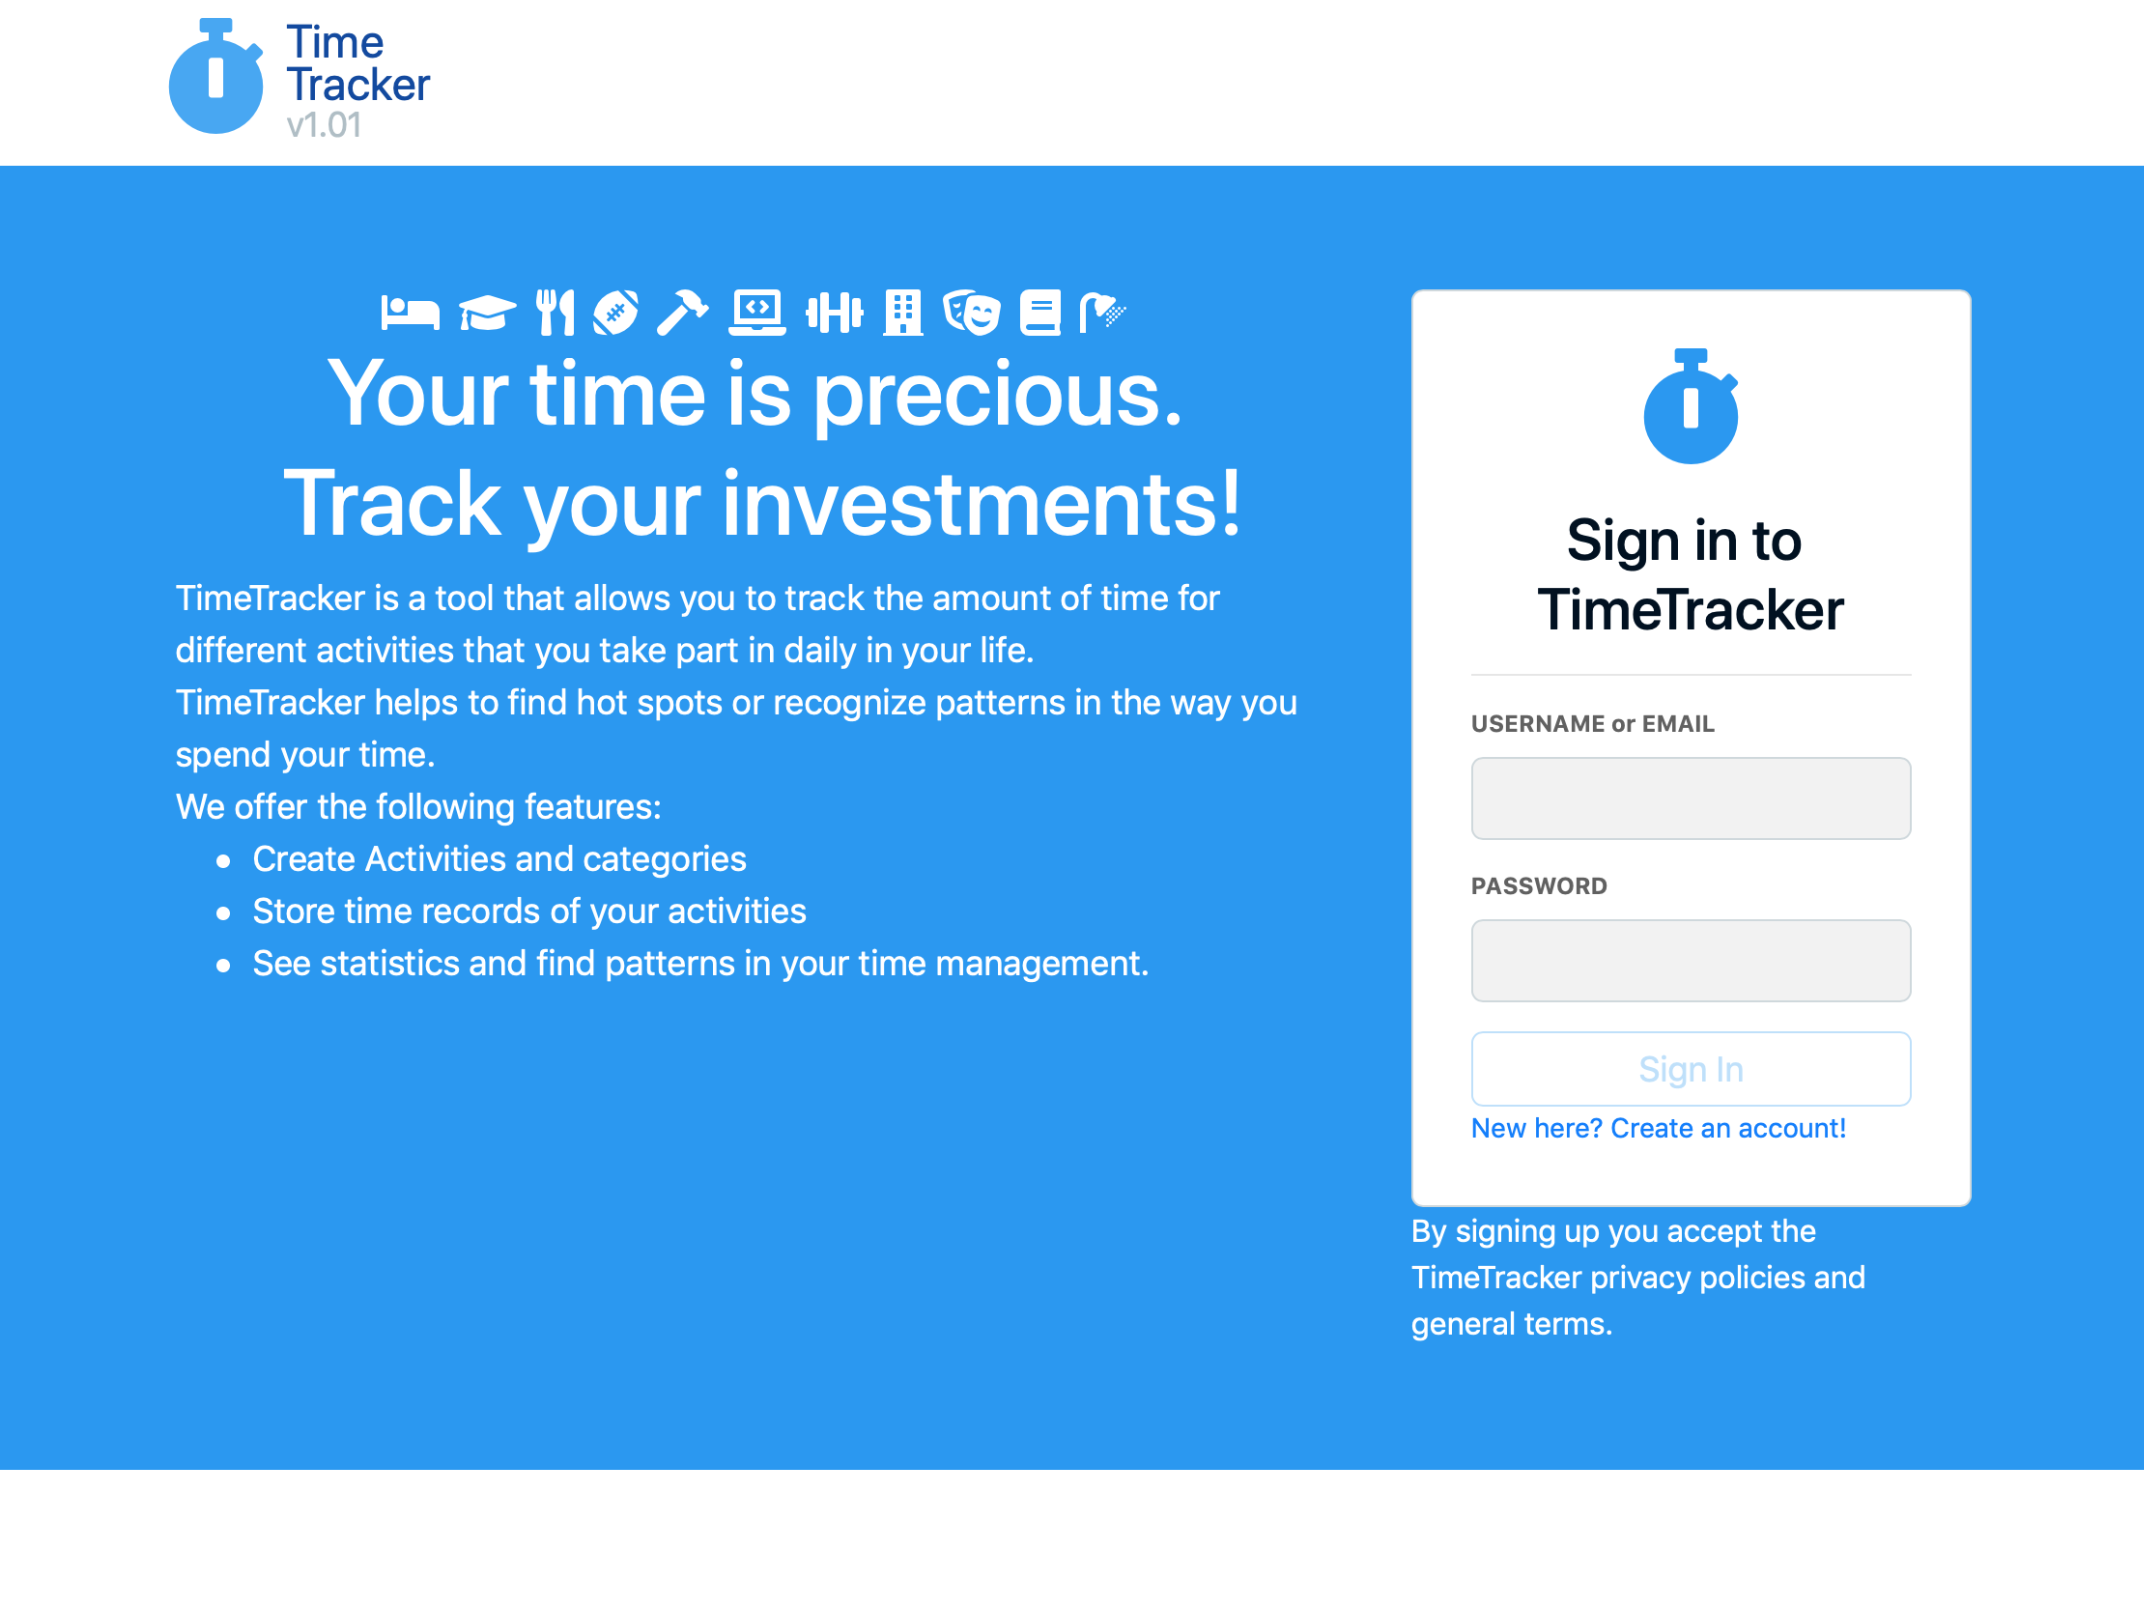
\includegraphics[width=1.15\linewidth]{login.png}
 	\caption{Login}
 	\label{fig:login}
 \end{figure}

Willkommen bei TimeTracker! Auf unserer Startseite (Abb. \ref{fig:login}) kannst du dich mit deinen Benutzerdaten einloggen.  
Du hast noch kein Benutzerkonto? Kein Problem, unterhalb des \textit{Sign In} Buttons ist ein Link, der zur Registrierung führt.
 

\begin{figure}[H]
	\hspace{-1.5cm}
	\centering
	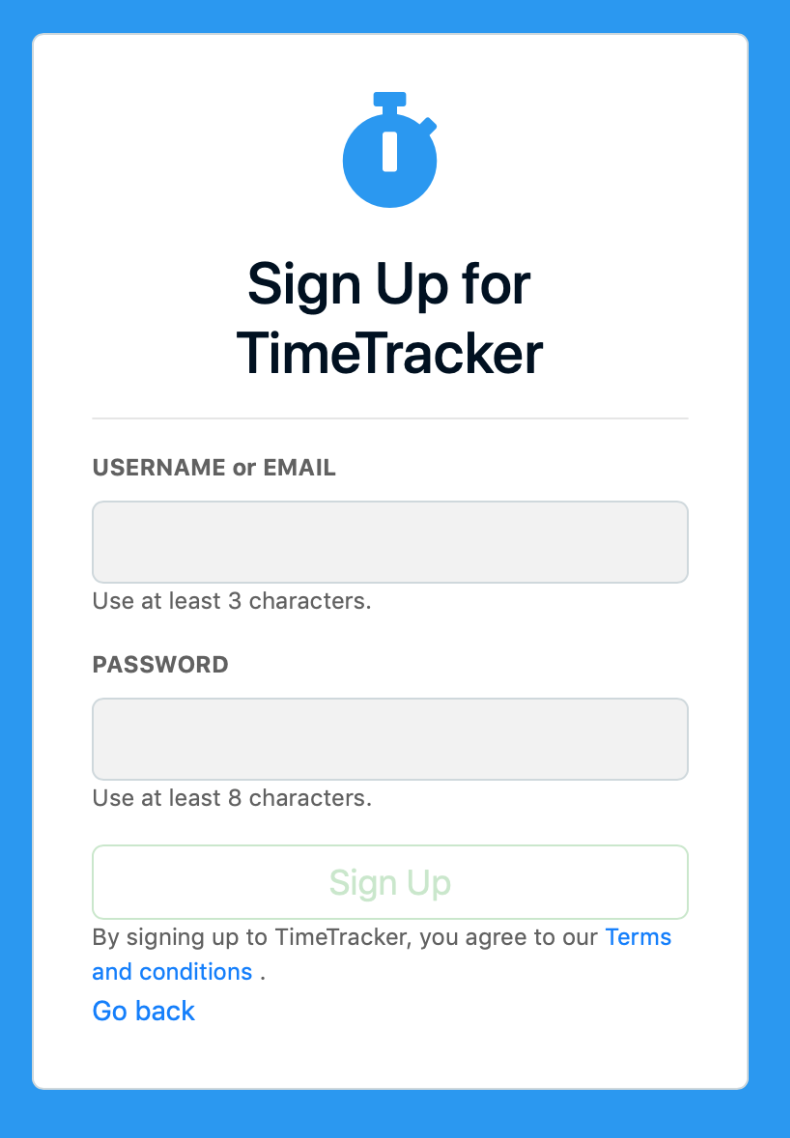
\includegraphics[scale=0.5]{register.png}
	\caption{Registrieren}
	\label{fig:register}
\end{figure}
%\newpage
%\begin{wrapfigure}{l}{0.5\textwidth}
%		\hspace{-1.5cm}
%		\centering
%		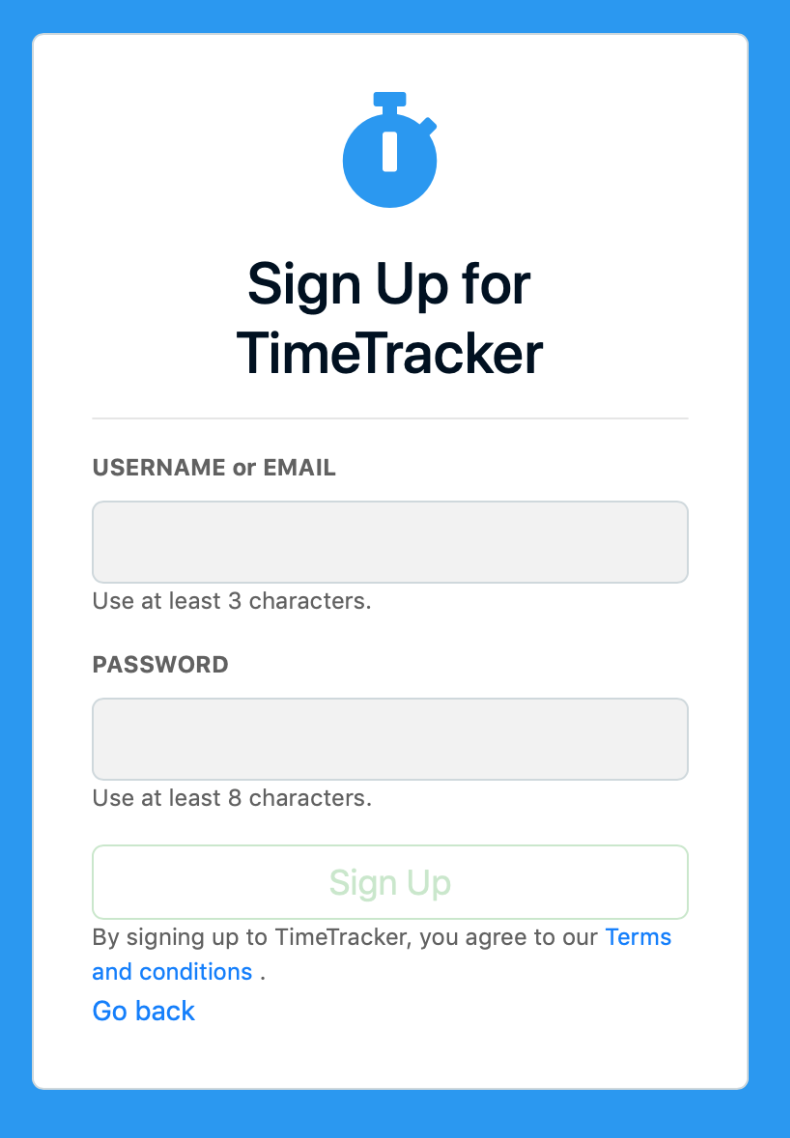
\includegraphics[width=0.38\textwidth]{register.png}
%		\caption{Registrieren}
%		\label{fig:register}
%\end{wrapfigure}

Um sich zu registrieren, wähle einen Usernamen sowie ein Passwort und klicke dann auf "Sign Up". Beachte bitte, dass das Passwort mindestens 8 Zeichen lang sein muss. Bitte merke Dir deine ausgewählten Credentials, da bislang noch keine Registrierungsbestätigung per Mail versendet wird.
Nachdem Du dich erfolgreich registriert haben, wirst Du wieder auf unsere Startseite (Abb. \ref{fig:login}) geleitet, wo Du dich ab sofort mit Deinen Nutzerdaten anmelden können. 

Wenn Du einmal angemeldet bist, kannst Du dich jederzeit mit einem Klick auf \textit{Logout} oben rechts wieder abmelden.

\subsection{TimeTracken}

Wenn Du dich das erste mal einloggst, sind noch keine Aktivitäten vorhanden. 
Aktivitäten sind alltägliche Aktionen, für die Du die Zeit trackst, die Du in sie investierst. Zum Beispiel Lernen, Reisen, Einkaufen, Sport treiben und so weiter. 
Füge einfach eine neue Aktivität hinzu, in dem Du auf \textit{+ New Activity} klickst (Abb. \ref{fig:no_activity}). 

\begin{figure}[H]
	\hspace{-1.5cm}
	\centering
	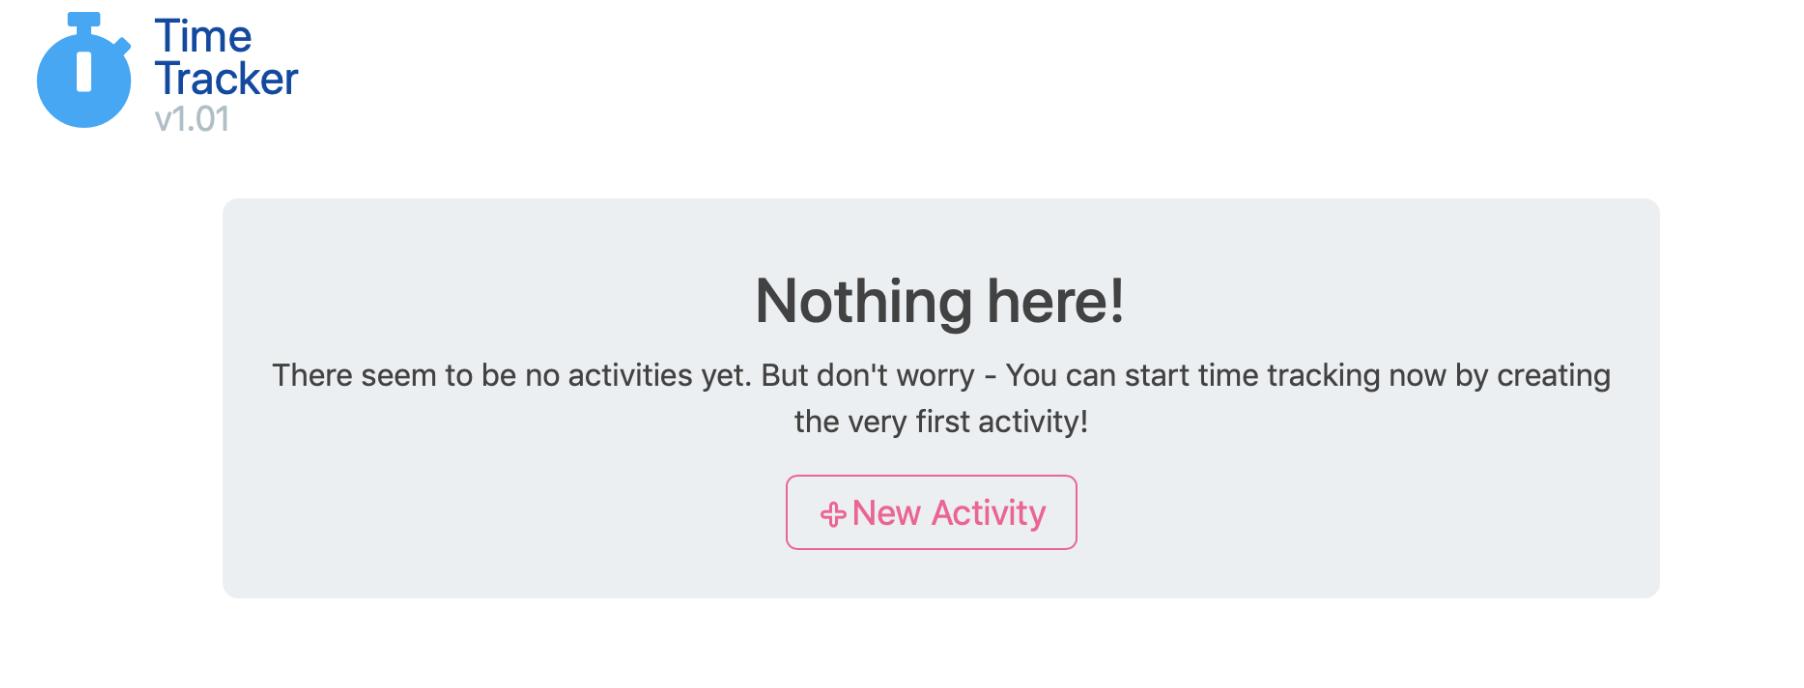
\includegraphics[scale=0.5]{no_activity.png}
	\caption{Keine Aktivitäten angelegt}
	\label{fig:no_activity}
\end{figure}

\begin{figure}[H]
	\hspace{-1.5cm}
	\centering
	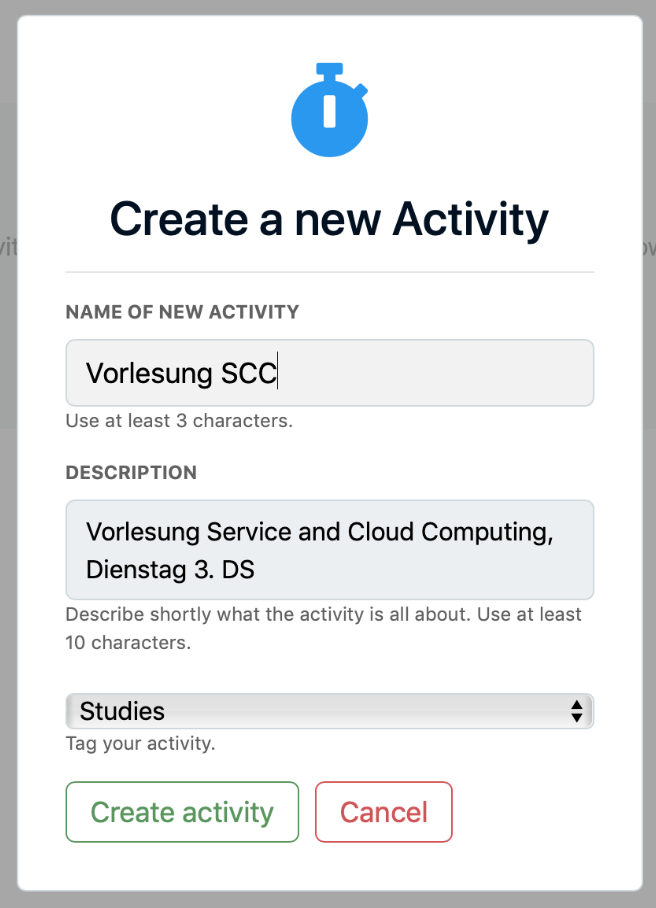
\includegraphics[scale=0.5]{create_activity.png}
	\caption{Aktivität anlegen}
	\label{fig:create_activity}
\end{figure}

Nun kannst Du die Aktivität genauer beschreiben (Abb. \ref{fig:create_activity}. 
Gib ihr einen Namen und eine Beschreibung, damit Du später weißt, wofür Du sie angelegt hast. 
Der Name darf keine Umlaute wie \glqq Ä, Ö, Ü\grqq{}  enthalten und die Beschreibung muss mindeste 10 Zeichen lang sein. 
Danach verbindest Du deine Aktivität mit einem Tag. Tags helfen Dir dabei, deine Activities zu kategorisieren.
Jede Aktivität hat ein Tag und dadurch eine Zuordnung zu einem Deiner Lebensbereiche. 
Tags sind beispielsweise Studies, Sport und Relax. 
Mit Hilfe der Tags kannst Du später schauen, wie viel Sport du gemacht hast, auch wenn Du deine Zeit in den Aktivitäten "Schwimmen" und "Rad fahren" aufgenommen hast. 


\begin{figure}[H]
	\hspace{-1.5cm}
	\centering
	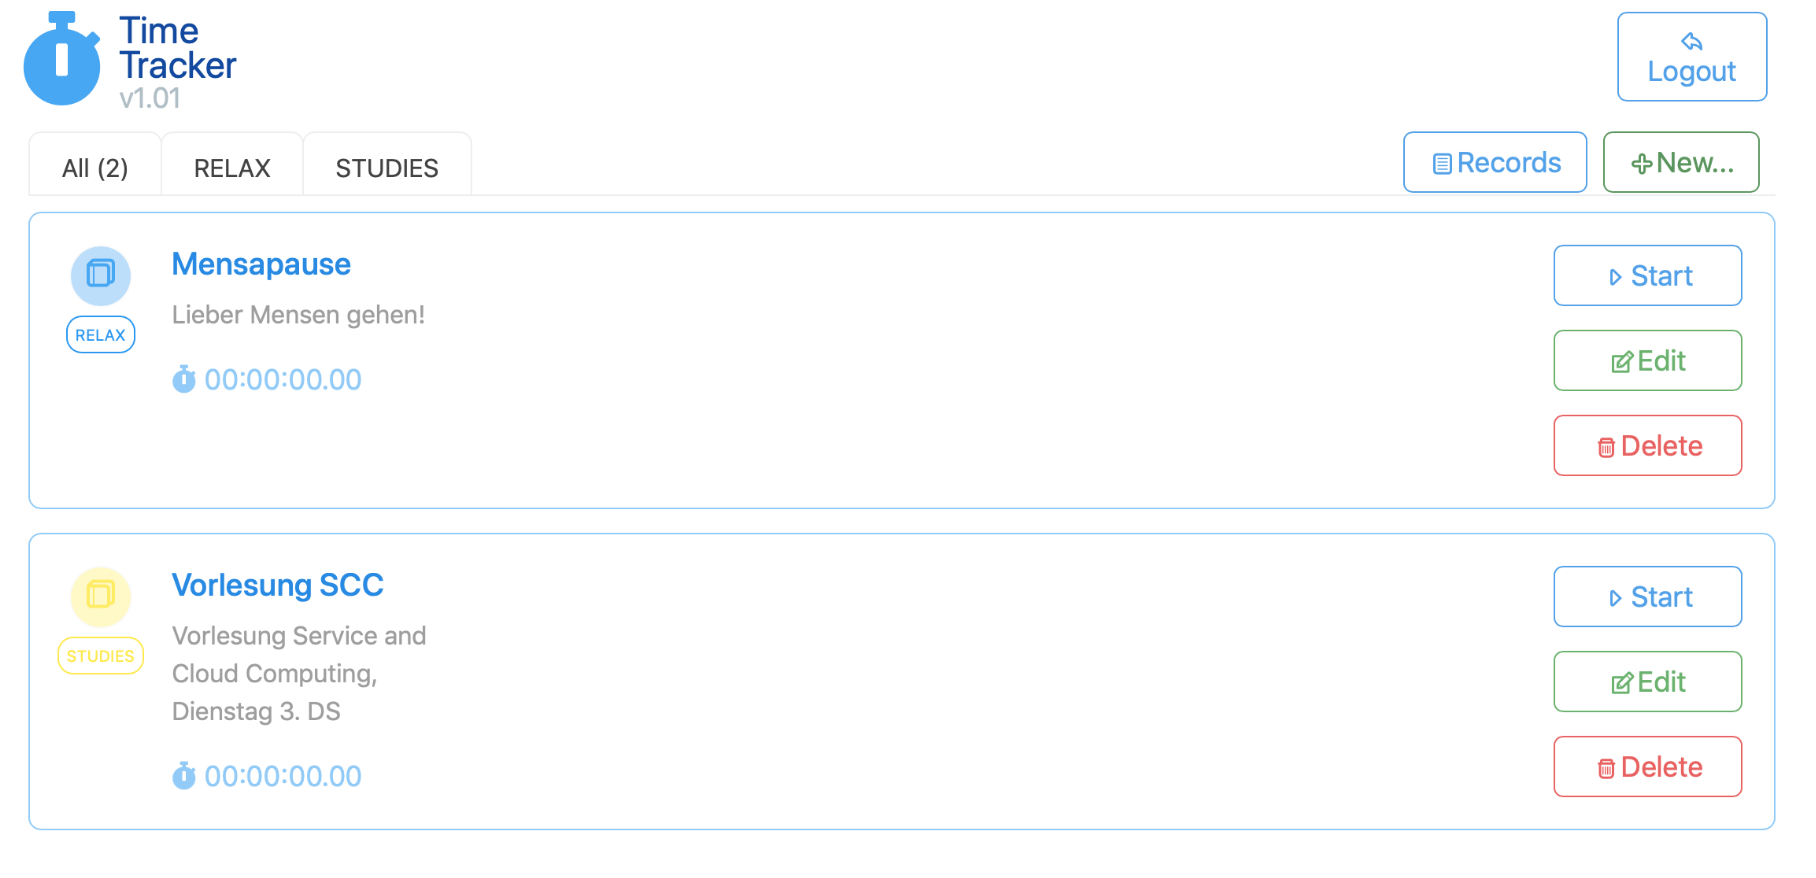
\includegraphics[scale=0.5]{activitys.png}
	\caption{Übersicht: Aktivitäten}
	\label{fig:activitys}
\end{figure}

Nun hast Du Aktivitäten und eine Übersicht (Abb. \ref{fig:activitys}. Hier kannst Du mit einem Klick auf  \textit{Start} ein Record beginnen. Records sind die einzelnen Aufnahmen, die Du machst, um investierte Zeit zu tracken. Summiert ergeben sie die gesamte Zeit, die du für eine Aktivität aufbringst. Nach einem Klick auf "Start" wirst Du sehen, dass die Stopuhr blinkt und die Zeit läuft. 
Mit einem Klick auf den selben Button stoppst du das Tracking deiner Aktivität und beendest den Record. Die Zeit des Records wird dir nun angezeigt.
Du kannst dich zwischendurch auch abmelden oder von einem anderen Gerät aus einloggen, die Aufnahme geht einfach weiter. 

Mit dem Button \textit{+ New} kannst du weitere Aktivitäten anlegen und mit dem Button \textit{Delete} die jeweilige auch wieder löschen. In dem du auf \textit{Edit} klickst kannst Du Namen, Beschreibung und Tag deiner Activities anpassen.

Wenn du auf einem Desktop TimeTracker nutzt, kannst Du über die Reiter oben die Ansicht nach Tags filtern. 

\begin{figure}[H]
	\hspace{-1.5cm}
	\centering
	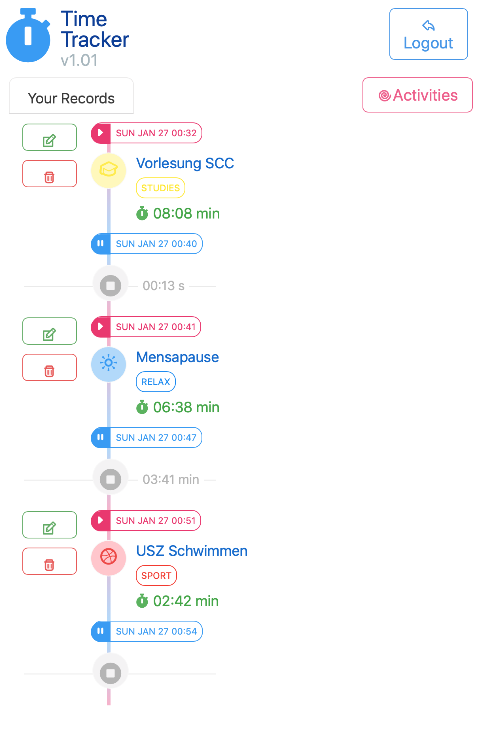
\includegraphics[scale=0.5]{records_new.png}
	\caption{Aufgenommene Records}
	\label{fig:records}
\end{figure}

Wenn du \textit{Records} anwählst, kommst Du zu einer Übersicht all deiner Zeitaufnahmen (Abb. \ref{fig:records}). Hier kannst Du genau sehen, wie viel Zeit Du für welche Aktivität investiert hast. Außerdem kannst Du von hier aus auch Records löschen.

